\documentclass[a4paper,12pt]{book}
\usepackage{natbib}

\usepackage{../../src/fancyhdr}
\usepackage{../../src/geometry}
\usepackage{../../src/graphicx}
\usepackage{../../src/hlundef}
\usepackage{../../src/tesis}
\usepackage{../../src/macro}
%\usepackage[spanish, es-ucroman]{babel}
\usepackage[english]{babel}
\usepackage[utf8]{inputenc}
%\usepackage{fancyhdr}
%\usepackage{graphicx}
%\usepackage[inner=3.0cm,outer=2.5cm,top=3cm,bottom=3cm]{geometry}
%\usepackage{hlundef}
%\usepackage{tesis}
\usepackage[printonlyused]{acronym}
\usepackage{breakcites}
\usepackage{color,soul}
\usepackage{ae}
\usepackage[usenames,dvipsnames,table,xcdraw]{xcolor}
\usepackage{amsmath}
\usepackage{multirow}
\usepackage[inline]{enumitem}
\usepackage{tikz,pgfplots,pgfplotstable}
\usepackage{capt-of}
\usepackage{csvsimple}

\usepackage{caption}
\usepackage{subcaption}
\usepackage{booktabs}
\usepackage{enumitem}
\usepackage[colorinlistoftodos]{todonotes}
\usepackage{mathrsfs}
\newtheorem{proposicion}{Proposición}[section]
\usepackage{amsfonts}
\usepackage{amssymb}
\usepackage{xspace}
\usepackage{array}
\usepackage{etoolbox}
\usepackage[group-separator={,}]{siunitx}

\usepackage{import}


\usepackage{booktabs}
\newcommand{\ra}[1]{\renewcommand{\arraystretch}{#1}}

\setcounter{secnumdepth}{3}

\usepackage{filecontents,pgfplots,pgfplotstable}
\pgfplotsset{compat=1.13}
\usepgfplotslibrary{colormaps}

\usepackage{sidecap}
\sidecaptionvpos{figure}{b}
\sidecaptionvpos{table}{b}

\usepackage{natbib}
\setcitestyle{round}
%\bibliographystyle{apabrahand}
\usepackage[colorlinks=true]{hyperref}
\hypersetup{citecolor=blue}
\hypersetup{urlcolor=red}
\hypersetup{linkcolor=purple}

\usepackage{tikz-qtree}
\usepackage{arydshln}
\usetikzlibrary{shapes.geometric, arrows, decorations.pathreplacing, shadows,trees, positioning, calc, tikzmark, spy, mindmap, matrix}
\tikzstyle{roundedFrame} = [rectangle, text centered, rounded corners, draw=gray]
\tikzstyle{input} = [rectangle,text centered, draw=none]
\tikzstyle{emptyFrame} = [rectangle,text centered, draw=white]
\tikzstyle{frame} = [rectangle, text centered, draw=gray]
\tikzstyle{arrow} = [thick,->,>=stealth]

\usepackage{pifont} % DING


%%%%%%%%%%% Extra commands %%%%%%%%%%%%%%
\newcommand{\myparagraph}[1]{\smallskip\noindent\textbf{#1}\space}
\newcommand{\ie}{\textit{i.e.},\xspace}
\newcommand{\eg}{\textit{e.g.},\xspace}
\newcommand{\ea}{\textit{et al.}\xspace}
\newcommand{\etc}{\textit{etc.}}

\definecolor{pastelblue}{rgb}{0.68, 0.78, 0.81}
\definecolor{pastelorange}{rgb}{1.0, 0.7, 0.28}
\definecolor{pastelyellow}{rgb}{0.99, 0.99, 0.59}
\definecolor{pastelred}{rgb}{1.0, 0.41, 0.38}
\definecolor{pastelgreen}{rgb}{0.47, 0.87, 0.47}
\definecolor{error}{rgb}{1.0, 0.41, 0.38} % red
\definecolor{note}{rgb}{0.99, 0.99, 0.59} % yellow
\definecolor{info}{rgb}{0.68, 0.78, 0.81} % blue
\definecolor{tip}{rgb}{0.47, 0.87, 0.47} % green

\begin{document}
    % 
\chapter{Safe and near optimal controller synthesis}

\label{ch:proposal}
In this part, we choose as a case of study an \emph{Hybrid Solar Water
Heating}, because this system link up important condition to implement the
methodology described in this work. Firstly we have agents, who interact with 
the system, adding uncontrollables modes of operations also some controllable
variables in the system that allow to model as stochastic hybrid game.

The first part is about mathematical modelling using heat transfer
theory and fluids dynamics to get temperature dinamics and then 
to define the parameters that determine the system with some
assumptions to facilate the analysis.

\section{Case study}
In this section, I test the proposed methodology for solving safe and near optimal controller synthesis 
for stochastic hybrid games.


\tikzset{every picture/.style={line width=0.75pt}} %set default line width to 0.75pt        

\begin{tikzpicture}[x=0.75pt,y=0.75pt,yscale=-1,xscale=1]
%uncomment if require: \path (0,300); %set diagram left start at 0, and has height of 300

%Rounded Rect [id:dp3454362135099034] 
\draw   (203,113.4) .. controls (203,105.45) and (209.45,99) .. (217.4,99) -- (282.1,99) .. controls (290.05,99) and (296.5,105.45) .. (296.5,113.4) -- (296.5,156.6) .. controls (296.5,164.55) and (290.05,171) .. (282.1,171) -- (217.4,171) .. controls (209.45,171) and (203,164.55) .. (203,156.6) -- cycle ;
%Straight Lines [id:da8670184653139519] 
\draw    (232.5,128) -- (175.5,128.97) ;
\draw [shift={(173.5,129)}, rotate = 359.03] [color={rgb, 255:red, 0; green, 0; blue, 0 }  ][line width=0.75]    (10.93,-3.29) .. controls (6.95,-1.4) and (3.31,-0.3) .. (0,0) .. controls (3.31,0.3) and (6.95,1.4) .. (10.93,3.29)   ;

%Image [id:dp1573774251550818] 
\draw (329.75,151.22) node  {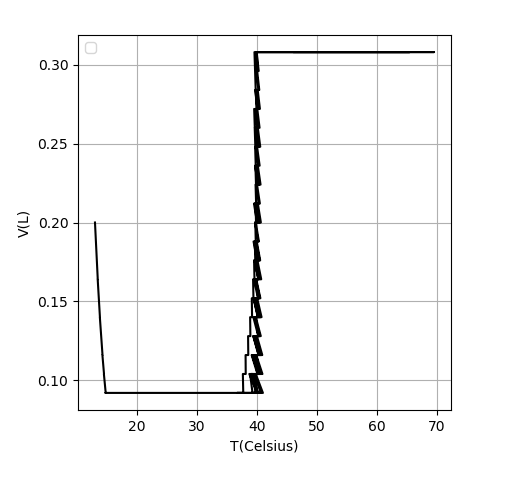
\includegraphics[width=391.13pt,height=232.5pt]{content/ch04/5.png}};
%Straight Lines [id:da756821456781489] 
\draw    (360.5,151.22) -- (442.5,150.24) ;
\draw [shift={(444.5,150.22)}, rotate = 539.3199999999999] [color={rgb, 255:red, 0; green, 0; blue, 0 }  ][line width=0.75]    (10.93,-3.29) .. controls (6.95,-1.4) and (3.31,-0.3) .. (0,0) .. controls (3.31,0.3) and (6.95,1.4) .. (10.93,3.29)   ;


%Straight Lines [id:da9580285561891552] 
\draw    (228.5,102.22) -- (302.5,101.24) ;
\draw [shift={(304.5,101.22)}, rotate = 539.25] [color={rgb, 255:red, 0; green, 0; blue, 0 }  ][line width=0.75]    (10.93,-3.29) .. controls (6.95,-1.4) and (3.31,-0.3) .. (0,0) .. controls (3.31,0.3) and (6.95,1.4) .. (10.93,3.29)   ;

%Straight Lines [id:da9281060785864365] 
\draw    (389.5,67.22) -- (430.5,67.22) ;
\draw [shift={(432.5,67.22)}, rotate = 180] [color={rgb, 255:red, 0; green, 0; blue, 0 }  ][line width=0.75]    (10.93,-3.29) .. controls (6.95,-1.4) and (3.31,-0.3) .. (0,0) .. controls (3.31,0.3) and (6.95,1.4) .. (10.93,3.29)   ;

%Straight Lines [id:da47053369422446445] 
\draw    (261.5,79.22) -- (294.5,79.22) ;
\draw [shift={(296.5,79.22)}, rotate = 180] [color={rgb, 255:red, 0; green, 0; blue, 0 }  ][line width=0.75]    (10.93,-3.29) .. controls (6.95,-1.4) and (3.31,-0.3) .. (0,0) .. controls (3.31,0.3) and (6.95,1.4) .. (10.93,3.29)   ;

%Shape: Circle [id:dp11314595015500317] 
\draw  [color={rgb, 255:red, 0; green, 0; blue, 0 }  ,draw opacity=1 ][fill={rgb, 255:red, 155; green, 155; blue, 155 }  ,fill opacity=1 ] (532.5,92.75) .. controls (532.5,88.19) and (536.19,84.5) .. (540.75,84.5) .. controls (545.31,84.5) and (549,88.19) .. (549,92.75) .. controls (549,97.31) and (545.31,101) .. (540.75,101) .. controls (536.19,101) and (532.5,97.31) .. (532.5,92.75) -- cycle ;

% Text Node
\draw (463,133) node   {$kA_{t}( T_{cont} -T_{env})$};
% Text Node
\draw (193,97) node   {$A_{c}( I_{env})$};
% Text Node
\draw (474,48) node   {$m( T_{cont} -T_{in})$};
% Text Node
\draw (339,116) node   {$T_{cont}$};
% Text Node
\draw (568,89) node   {$T_{env}$};
% Text Node
\draw (539,278) node   {$T_{in}$};
% Text Node
\draw (276,60) node   {$P_{aux}$};
% Text Node
\draw (540,217) node   {$T_{cont}$};


\end{tikzpicture}



\subsection{Setup system}

\begin{equation}
    \factorheat\mcont\frac{d}{dt}\tcont =  Q_{input,1} + Q_{input,2} - Q_{loss,1} -  Q_{loss,2}
\end{equation}

\begin{equation}
    Q_{input,1} =   A_c\cdot\irradiance
\end{equation}

\begin{equation}
    Q_{input,2} =   \haux
\end{equation}

\begin{equation}
    Q_{loss,1} =  \factorheat \flowin (\tcont-\tin)
\end{equation}

\begin{equation}
    Q_{loss,2} =  k_c A_t (\tcont-\tenv)
\end{equation}

\subsection{State Variables}

\begin{itemize}
\item
$\tcont$ the temperature of the container in \si{\degreeCelsius}
\item
$\vcont$ the volume of the container in \si{\metre^3}

\end{itemize}

\subsection{Constants}
\begin{itemize}
\item 
$\factorheat$ The factor heat of the water in \si{\joule\per\degreeCelsius\per\kilogram}
\item
$\flowin$ Mass flow rate input/output  \si{\kilogram\per\second}
\item
$\mcont$ the mass of the container in \si{\kilogram}
\item
$A_c$ Area of colector in \si{\metre^2}
\item
$A_t$ Area of total of surface in \si{\metre^2}
\item
$k_c$ Conduction coeficient \si{\watt\per\metre\per\degreeCelsius}
\item
$\haux$ Auxiliary heat power in \si{\watt}

\end{itemize}

\subsection{Input Variables}
\begin{itemize}
\item
Valve for output water state = $\left\lbrace on,off \right\rbrace $
\item
Volume states = $\left\lbrace1,2,3\right\rbrace $
\item
Auxiliary heat state = $\left\lbrace on,off \right\rbrace $


\end{itemize}

\subsection{Disturbance Variables}
\begin{itemize}
\item 
$\tin$ the temperature of water input/output in \si{\degreeCelsius}
\item
$\irradiance$ the irradiance in \si{\watt\per\square\metre}
\item
$\tenv$ the outside temperature in \si{\degreeCelsius}
\end{itemize}

\begin{table}[ht]
\centering
\caption{Parameter values.}
\begin{tabular}[t]{lcc}
\hline
Parameter && Values\\
\hline
$C_e$&&4186\si{\joule\per\degreeCelsius\per\kilogram}\\
$\flowin$&&0.1\si{\kilogram\per\second}\\
$\mcont$&&100\si{\kilogram}\\
$A_c$&&1\si{\metre^2}\\
$A_t$&&5.5557\si{\metre^2}\\
$k_c$&&16\si{\watt\per\metre\per\degreeCelsius}\\
$\haux$&&1000\si{\joule\per\second}\\
%$A_{pist}$&&1\si{\metre^2}\\
%$v_{pist}$&&0.1\si{\metre\per\second}\\
\hline
\end{tabular}
\label{table} 
\end{table}%

%\begin{figure}[h]
%  \centering
%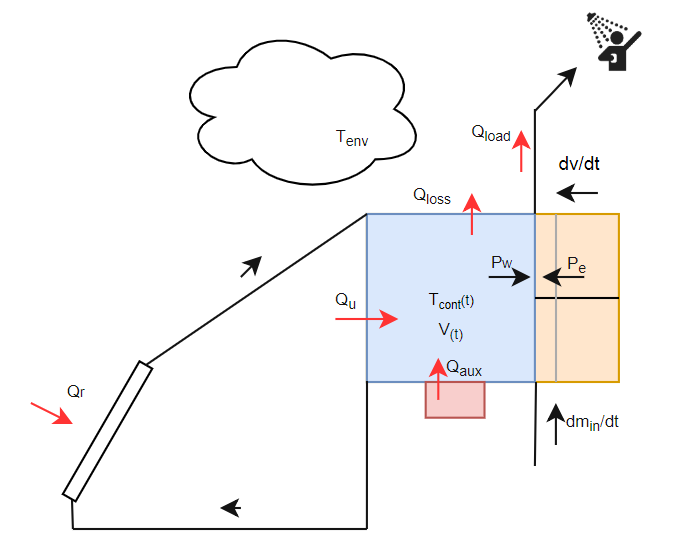
\includegraphics[scale=0.6]{images/SWH.png}
%  \caption{Hybrid Solar Water Heating Diagram}  
%  \label{fig:systemSetup}
%\end{figure}

\newpage

\section{Hybrid solar water heating as a Sthocastic Hybrid Game}
The hybrid solar water heating scenario with 12 modes of operations is
defined  like this: $\mathcal{G}_{n,m} = (\mathcal{C,U,X,F},\delta)$, 
where the controller $\mathcal{C}$ has a finite set of controllable modes,
given by resistance state ${r \in \mathbb{B}}$ and piston position $p \in 
\left\lbrace1,2,3\right\rbrace $. The environment $\mathcal{U}$ has a finite  
set of uncontrollable modes $v \in \mathbb{B} $, that means the valve state 
for opening/closing water aperture. We assume that $\mathcal{U}$ given
$\delta$ can switch among modes with equal probability at every period. 
The state variables in $\mathcal{X}$ are given by $\left\lbrace
T,E,V \right\rbrace $, container temperature, energy used and container volumen
respectively.

Given the container temparature and volume, a controllable modes $r \in \mathbb{B}$
and $p \in \left\lbrace1,2,3\right\rbrace $ and uncontrollable mode
$v \in \mathbb{B} $ and a time delay $\tau$.

%\begin{equation}
%  \frac{d}{dt}\tcont(t) = \constone(\tenv-\tcont)+\consttwo\tirrad+
%  \constthree\taux+\constfour(\tcont-\tin)
%\end{equation}

\begin{equation}
    \begin{aligned}
\frac{d}{dt}\tcont = \frac{1}{V(t)} [ -\constone(\tcont-\tenv)
- p \consttwo(\tcont-\tin) \\
- f \constthree(pV_{min} - \vcont)(\tcont-\tin)
+ \constfour\irradiance+ 
r \constfive ]
    \end{aligned}
\label{temperature-equation}    
\end{equation}

\begin{equation}
\frac{d}{dt}\vcont = pV_{min} - \vcont; \quad
\label{volume-equation}
\end{equation}

\begin{equation} 
\frac{d}{dt}E_{used} =  r \constthree ;
\label{Energy-equation}
\end{equation}

The equation \ref{temperature-equation} has some constants $\left\lbrace 
\constone, \consttwo, \constthree, \constfour \right\rbrace $ this
parameters are computed with the parameteres defines in table \ref{table} for specific Hybrid Solar Water Heating
are equal to $\left\lbrace 2.44e^{-5},  4.77e^{-6}
, 0.0024, 0.01  \right\rbrace$ respectively.


\section{Simulations}

near optimal controller
near optimal controller
near optimal controller
near optimal controller
near optimal controller

\begin{minipage}{\linewidth}
\begin{center}
\includegraphics[width=1.0\linewidth]{content/ch04/1}
\captionof{figure}{An example image not including a Wombat}
\end{center}
\end{minipage}

The Figure environment "floats" to find an optimal position on the page. When you begin a figure, you can use the options [htbp!] to specify whether the figure should go "here", the "top" of this page, the "bottom" of this page, or a special "page" reserved for floats. LaTeX, in its infinite wisdom, will sometimes prevent you from putting a figure in an "ugly" place, but you can (sort of) override its decision using the "!" option. When you haven't used any option, the environment assumes that you provided [tbp], and it's choosing to put the figure at the top of the page, above where your section goes. So using


\section{Results}
this is 
%\subsection{Experimental Results}
%\begin{figure}[h]
%  \centering
%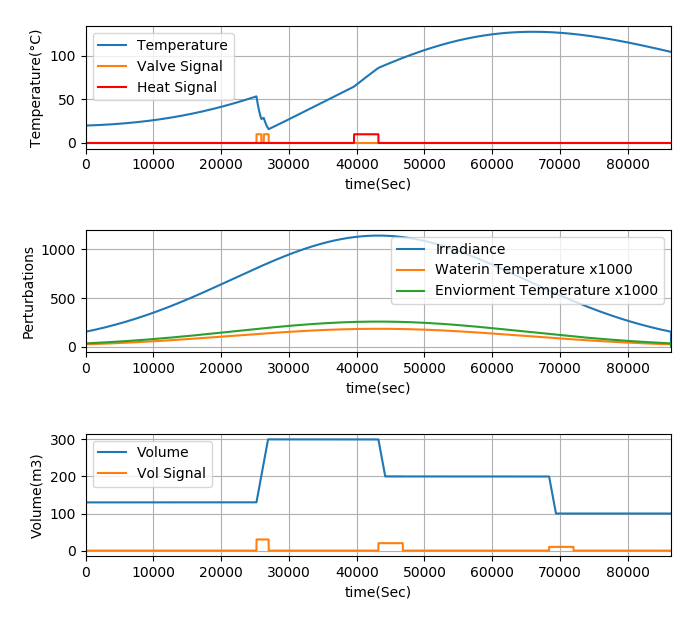
\includegraphics[scale=0.8]{images/result.png}
%  \caption{Hybrid Solar Water Heatin response}
%\label{fig:systemSetup}
%\end{figure}
% \bibliography{../../thesis-doc}{} % m02 Error! -> mO2 (Ok)

%\bibliographystyle{../src/apabrahand}
 
    
    \chapter{Hybrid Solar Water heating}
    \label{ch:proposal}

    In this part, we choose as a case of study an \emph{Hybrid Solar Water
    Heating}, because this system link up important condition to implement the
    methodology described in this work. Firstly we have agents, who interact with 
    the system, adding uncontrollables modes of operations also some controllable
    variables in the system that allow to model as stochastic hybrid game.

    The first part is about mathematical modelling using heat transfer
    theory and fluids dynamics to get temperature dinamics and then 
    to define the parameters that determine the system with some
    assumptions to facilate the analysis.

    \section{System Setup}

    
\tikzset{every picture/.style={line width=0.75pt}} %set default line width to 0.75pt        

\begin{tikzpicture}[x=0.75pt,y=0.75pt,yscale=-1,xscale=1]
%uncomment if require: \path (0,300); %set diagram left start at 0, and has height of 300

%Rounded Rect [id:dp3454362135099034] 
\draw   (203,113.4) .. controls (203,105.45) and (209.45,99) .. (217.4,99) -- (282.1,99) .. controls (290.05,99) and (296.5,105.45) .. (296.5,113.4) -- (296.5,156.6) .. controls (296.5,164.55) and (290.05,171) .. (282.1,171) -- (217.4,171) .. controls (209.45,171) and (203,164.55) .. (203,156.6) -- cycle ;
%Straight Lines [id:da8670184653139519] 
\draw    (232.5,128) -- (175.5,128.97) ;
\draw [shift={(173.5,129)}, rotate = 359.03] [color={rgb, 255:red, 0; green, 0; blue, 0 }  ][line width=0.75]    (10.93,-3.29) .. controls (6.95,-1.4) and (3.31,-0.3) .. (0,0) .. controls (3.31,0.3) and (6.95,1.4) .. (10.93,3.29)   ;

%Image [id:dp1573774251550818] 
\draw (329.75,151.22) node  {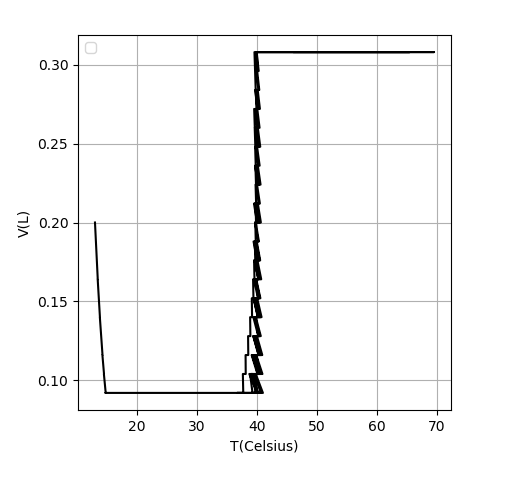
\includegraphics[width=391.13pt,height=232.5pt]{content/ch04/5.png}};
%Straight Lines [id:da756821456781489] 
\draw    (360.5,151.22) -- (442.5,150.24) ;
\draw [shift={(444.5,150.22)}, rotate = 539.3199999999999] [color={rgb, 255:red, 0; green, 0; blue, 0 }  ][line width=0.75]    (10.93,-3.29) .. controls (6.95,-1.4) and (3.31,-0.3) .. (0,0) .. controls (3.31,0.3) and (6.95,1.4) .. (10.93,3.29)   ;


%Straight Lines [id:da9580285561891552] 
\draw    (228.5,102.22) -- (302.5,101.24) ;
\draw [shift={(304.5,101.22)}, rotate = 539.25] [color={rgb, 255:red, 0; green, 0; blue, 0 }  ][line width=0.75]    (10.93,-3.29) .. controls (6.95,-1.4) and (3.31,-0.3) .. (0,0) .. controls (3.31,0.3) and (6.95,1.4) .. (10.93,3.29)   ;

%Straight Lines [id:da9281060785864365] 
\draw    (389.5,67.22) -- (430.5,67.22) ;
\draw [shift={(432.5,67.22)}, rotate = 180] [color={rgb, 255:red, 0; green, 0; blue, 0 }  ][line width=0.75]    (10.93,-3.29) .. controls (6.95,-1.4) and (3.31,-0.3) .. (0,0) .. controls (3.31,0.3) and (6.95,1.4) .. (10.93,3.29)   ;

%Straight Lines [id:da47053369422446445] 
\draw    (261.5,79.22) -- (294.5,79.22) ;
\draw [shift={(296.5,79.22)}, rotate = 180] [color={rgb, 255:red, 0; green, 0; blue, 0 }  ][line width=0.75]    (10.93,-3.29) .. controls (6.95,-1.4) and (3.31,-0.3) .. (0,0) .. controls (3.31,0.3) and (6.95,1.4) .. (10.93,3.29)   ;

%Shape: Circle [id:dp11314595015500317] 
\draw  [color={rgb, 255:red, 0; green, 0; blue, 0 }  ,draw opacity=1 ][fill={rgb, 255:red, 155; green, 155; blue, 155 }  ,fill opacity=1 ] (532.5,92.75) .. controls (532.5,88.19) and (536.19,84.5) .. (540.75,84.5) .. controls (545.31,84.5) and (549,88.19) .. (549,92.75) .. controls (549,97.31) and (545.31,101) .. (540.75,101) .. controls (536.19,101) and (532.5,97.31) .. (532.5,92.75) -- cycle ;

% Text Node
\draw (463,133) node   {$kA_{t}( T_{cont} -T_{env})$};
% Text Node
\draw (193,97) node   {$A_{c}( I_{env})$};
% Text Node
\draw (474,48) node   {$m( T_{cont} -T_{in})$};
% Text Node
\draw (339,116) node   {$T_{cont}$};
% Text Node
\draw (568,89) node   {$T_{env}$};
% Text Node
\draw (539,278) node   {$T_{in}$};
% Text Node
\draw (276,60) node   {$P_{aux}$};
% Text Node
\draw (540,217) node   {$T_{cont}$};


\end{tikzpicture}


    \subsection{General Equation}

    \begin{equation}
    \factorheat\mcont\frac{d}{dt}\tcont =  Q_{input,1} + Q_{input,2} - Q_{loss,1} -  Q_{loss,2}
    \end{equation}

    \begin{equation}
        Q_{input,1} =   A_c\cdot\irradiance
    \end{equation}

    \begin{equation}
        Q_{input,2} =   \haux
    \end{equation}

    \begin{equation}
        Q_{loss,1} =  \factorheat \flowin (\tcont-\tin)
    \end{equation}

    \begin{equation}
        Q_{loss,2} =  k_c A_t (\tcont-\tenv)
    \end{equation}

    \subsection{State Variables}

    \begin{itemize}
    \item
    $\tcont$ the temperature of the container in \si{\degreeCelsius}
    \item
    $\vcont$ the volume of the container in \si{\metre^3}

    \end{itemize}

    \subsection{Constants}
    \begin{itemize}
    \item 
    $\factorheat$ The factor heat of the water in \si{\joule\per\degreeCelsius\per\kilogram}
    \item
    $\flowin$ Mass flow rate input/output  \si{\kilogram\per\second}
    \item
    $\mcont$ the mass of the container in \si{\kilogram}
    \item
    $A_c$ Area of colector in \si{\metre^2}
    \item
    $A_t$ Area of total of surface in \si{\metre^2}
    \item
    $k_c$ Conduction coeficient \si{\watt\per\metre\per\degreeCelsius}
    \item
    $\haux$ Auxiliary heat power in \si{\watt}

    \end{itemize}

    \subsection{Input Variables}
    \begin{itemize}
    \item
    Valve for output water state = $\left\lbrace on,off \right\rbrace $
    \item
    Volume states = $\left\lbrace1,2,3\right\rbrace $
    \item
    Auxiliary heat state = $\left\lbrace on,off \right\rbrace $


    \end{itemize}

    \subsection{Disturbance Variables}
    \begin{itemize}
    \item 
    $\tin$ the temperature of water input/output in \si{\degreeCelsius}
    \item
    $\irradiance$ the irradiance in \si{\watt\per\square\metre}
    \item
    $\tenv$ the outside temperature in \si{\degreeCelsius}
    \end{itemize}

    \begin{table}[ht]
    \centering
    \caption{Parameter values.}
    \begin{tabular}[t]{lcc}
    \hline
    Parameter && Values\\
    \hline
    $C_e$&&4186\si{\joule\per\degreeCelsius\per\kilogram}\\
    $\flowin$&&0.1\si{\kilogram\per\second}\\
    $\mcont$&&100\si{\kilogram}\\
    $A_c$&&1\si{\metre^2}\\
    $A_t$&&5.5557\si{\metre^2}\\
    $k_c$&&16\si{\watt\per\metre\per\degreeCelsius}\\
    $\haux$&&1000\si{\joule\per\second}\\
    %$A_{pist}$&&1\si{\metre^2}\\
    %$v_{pist}$&&0.1\si{\metre\per\second}\\
    \hline
    \end{tabular}
    \label{table} 
    \end{table}%

    %\begin{figure}[h]
    %  \centering
    %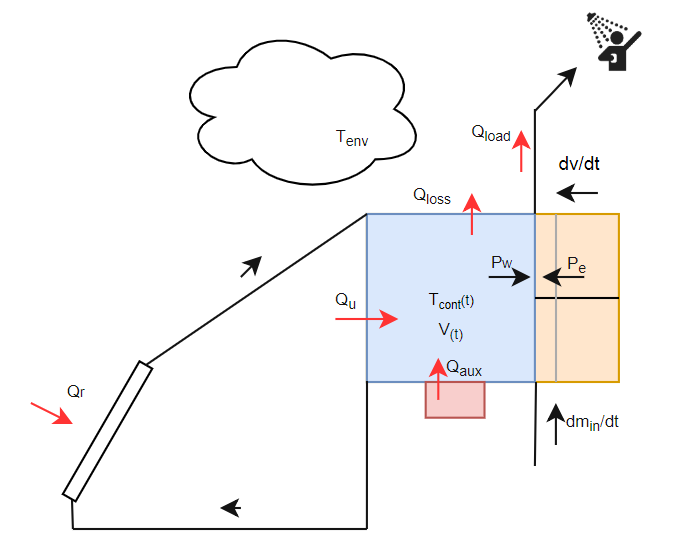
\includegraphics[scale=0.6]{images/SWH.png}
    %  \caption{Hybrid Solar Water Heating Diagram}  
    %  \label{fig:systemSetup}
    %\end{figure}

    \newpage

    \section{Hybrid solar water heating as a Sthocastic Hybrid Game}
    The hybrid solar water heating scenario with 12 modes of operations is
    defined  like this: $\mathcal{G}_{n,m} = (\mathcal{C,U,X,F},\delta)$, 
    where the controller $\mathcal{C}$ has a finite set of controllable modes,
    given by resistance state ${r \in \mathbb{B}}$ and piston position $p \in 
    \left\lbrace1,2,3\right\rbrace $. The environment $\mathcal{U}$ has a finite  
    set of uncontrollable modes $v \in \mathbb{B} $, that means the valve state 
    for opening/closing water aperture. We assume that $\mathcal{U}$ given
    $\delta$ can switch among modes with equal probability at every period. 
    The state variables in $\mathcal{X}$ are given by $\left\lbrace
    T,E,V \right\rbrace $, container temperature, energy used and container volumen
    respectively.

    Given the container temparature and volume, a controllable modes $r \in \mathbb{B}$
    and $p \in \left\lbrace1,2,3\right\rbrace $ and uncontrollable mode
    $v \in \mathbb{B} $ and a time delay $\tau$.

    %\begin{equation}
    %  \frac{d}{dt}\tcont(t) = \constone(\tenv-\tcont)+\consttwo\tirrad+
    %  \constthree\taux+\constfour(\tcont-\tin)
    %\end{equation}

    
    \begin{equation}
    \frac{d}{dt}\tcont =   \frac{1}{V(t)}  \constone(\tenv-\tcont)+ \frac{1}{V(t)} \consttwo\irradiance+  \frac{r}{V(t)} \constthree +  \frac{v}{V()} \constfour(\tin-\tcont)
    \label{temperature-equation}
    \end{equation}

    \begin{equation}
    \frac{d}{dt}\vcont = sgn(100p - \vcont); \quad
    \label{volume-equation}
    \end{equation}

    \begin{equation} 
    \frac{d}{dt}E_{used} =  r \constthree ;
    \label{Energy-equation}
    \end{equation}

    The equation \ref{temperature-equation} has some constants $\left\lbrace 
    \constone, \consttwo, \constthree, \constfour \right\rbrace $ this
    parameters are computed with the parameteres defines in table \ref{table} for specific Hybrid Solar Water Heating
    are equal to $\left\lbrace 2.44e^{-5},  4.77e^{-6}
    , 0.0024, 0.01  \right\rbrace$ respectively.


    \section{Simulations}


    \begin{figure}
        \includegraphics[width=\linewidth]{1.png}
        \caption{State Space.}
        \label{fig:1}
    \end{figure}

    \begin{figure}
        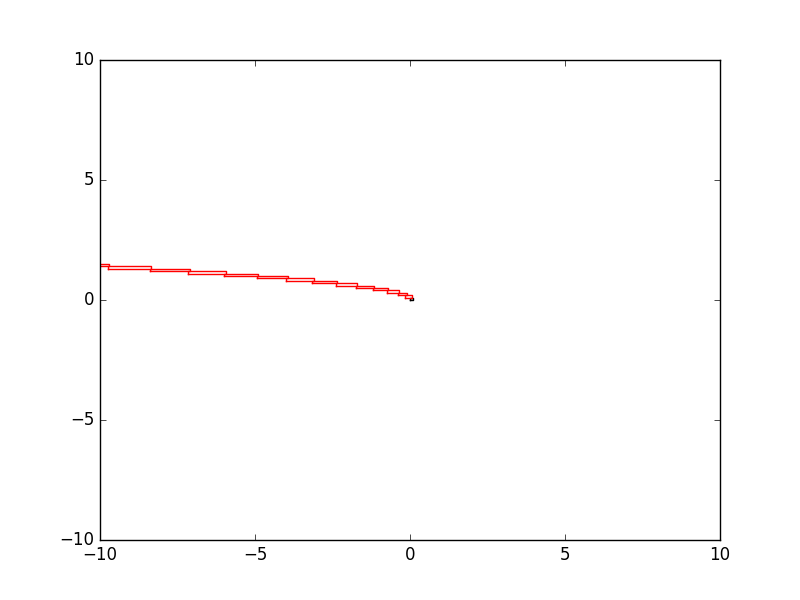
\includegraphics[width=\linewidth]{2.png}
        \caption{State Space 2.}
        \label{fig:1}
    \end{figure}


    \begin{figure}
        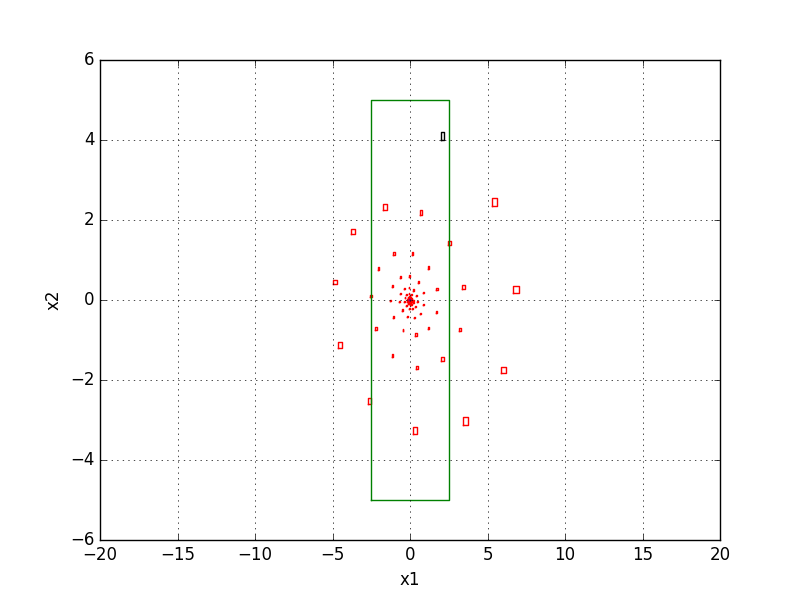
\includegraphics[width=\linewidth]{3.png}
        \caption{State Space 3.}
        \label{fig:1}
    \end{figure}


    %\subsection{Experimental Results}

    %\begin{figure}[h]
    %  \centering
    %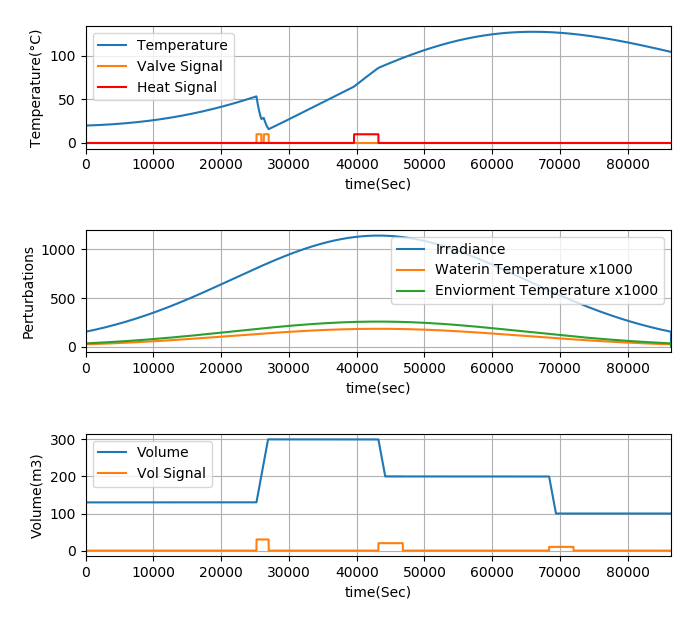
\includegraphics[scale=0.8]{images/result.png}
    %  \caption{Hybrid Solar Water Heatin response}
    
    %\label{fig:systemSetup}
    %\end{figure}



    % \bibliography{../../thesis-doc}{} % m02 Error! -> mO2 (Ok)
    \bibliographystyle{../src/apabrahand}
\end{document}